\subsubsection{UC10 - Visualizzazione lista \glossario{dizionario dati}}\label{UC10}

\begin{figure}[H]
  \centering
  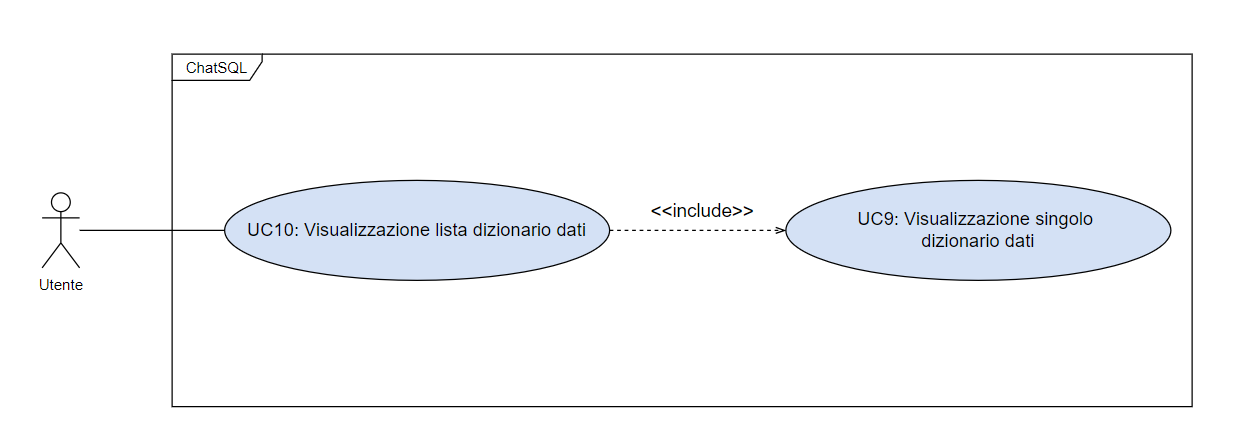
\includegraphics[width=0.90\textwidth]{assets/uc10.png}
  \caption{UC10}
\end{figure}

\paragraph*{Descrizione}
L’Utente visualizza la lista dei \glossario{dizionari dati} che sono stati caricati nel sistema.

\paragraph*{Attori principali}
Utente

\paragraph*{Precondizioni}
\begin{itemize}
  \item È presente almeno un \glossario{dizionario dati} nel sistema.  
\end{itemize}

\paragraph*{Postcondizioni}
\begin{itemize}
  \item L’Utente visualizza la lista completa dei \glossario{dizionari dati} nel sistema.
\end{itemize}

\paragraph*{Scenario principale}
\begin{enumerate}
  \item L’Utente decide di visualizzare i \glossario{dizionari dati} caricati;
  \item Viene esposta la lista dei \glossario{dizionari dati}.
\end{enumerate}

\paragraph*{Inclusione}
\begin{itemize}
  \item Visualizzazione singolo \glossario{dizionario dati} (\hyperref[UC9]{UC9}).
\end{itemize}

% Da aggiungere forse un UC per il fallimento di visualizzazione della lista
